\documentclass[10pt]{article}
\usepackage[utf8]{inputenc}
\usepackage[T1]{fontenc}
\usepackage{amsmath}
\usepackage{amsfonts}
\usepackage{amssymb}
\usepackage{mhchem}
\usepackage{stmaryrd}
\usepackage{graphicx}
\usepackage[export]{adjustbox}
\graphicspath{ {./images/} }

\title{Filtration Calculations }

\author{}
\date{}


\begin{document}
\maketitle
For the filtration process to work efficiently in the treatment plant, the operator needs to make sure everything is working according to the design criteria of the plant. Certain math calculations will help determine if and where there may be a problem with the filtration process.

\section{Flow Rate Through a Filter}
Flow rate through a filter can be determined by simply converting the gpd flow rate, as indicated on the flow meter. The gpm flow rate can be calculated by taking the meter flow rate (gpd) and dividing by $1440 \mathrm{~min} /$ day:

Flow rate, gpm $=\frac{\text { Flow rate, gpd }}{1440 \mathrm{~min} / \text { day }}$

\section{Example 1:}
The flow rate through a filter is $4.25$ MGD. What is this flow rate expressed as gpm?

Flow rate, gpm $=\frac{\text { Flow rate, gpd }}{1440 \mathrm{~min} / \text { day }}$

Flow rate, gpm $=\frac{4,250,000 \mathrm{gpd}}{1440 \mathrm{~min} / \text { day }}$

Flow rate, gpm $=2951 \mathrm{gpm}$
$$
\frac{4.25 \mathrm{MG}}{\text { day }} \times \frac{1,000,000 \mathrm{gal}}{1 \mathrm{MG}} \times \frac{1 \text { day }}{1440 \mathrm{~min}}=2951 \mathrm{gpm}
$$
You can work the problem above either way. All you need to do is convert the flow rate from MGD to gpm, which we've done before.

\section{Example 2:}
During a 70-hour filter run, a total of $22.4$ million gallons of water are filtered. What is the average flow rate through the filter in gpm during this filter run?

Flow rate, gpm $=\frac{\text { Total gallons produced }}{\text { Filter run, min }}$

Flow rate, gpm $=\frac{22,400,000 \mathrm{gal}}{70 \mathrm{hr} \times 60 \mathrm{~min} / \mathrm{hr}}$

Flow rate, gpm $=53333$ gpm Or you can break it down step by step. If you do not automatically look at $22.4 \mathrm{MG}$ and know that is the same as $22,400,000$ gal you can work it out with conversions to determine:
$$
22.4 \mathrm{MG} \times \frac{1,000,000 \mathrm{gal}}{1 \mathrm{MG}}=22,400,000 \mathrm{gal}
$$
You can also combine the filter run time like the equation above, or you can determine that before plugging it into the equation in the minute slot:

$70 \mathrm{hr} \mathrm{x} \frac{60 \mathrm{~min}}{1 \mathrm{hr}}=4,200 \mathrm{~min}$

Flow rate, gpm $=\frac{22,400,000 \mathrm{gal}}{4,200 \mathrm{~min}}$

Flow rate, gpm $=5333 \mathrm{gpm}$

Now, let's look at another problem dealing with flow rate through a filter. This time the question asks for the filter run time, so we will have to manipulate the equation to solve for the unknown component.

\section{Example 3:}
At an average flow rate of $4000 \mathrm{gpm}$, how long of a filter run, in hours, would be required to produce 25 MG of filtered water?

*Note: Write the equation as usual, fill in in the known data:
$$
\begin{aligned}
&\text { Flow rate, gpm }=\frac{\text { Total gallons produced }}{\text { Filter run, min }} \\
&4000 \text { gpm }=\frac{25,000,000 \text { gal }}{\text { Filter run, min }}
\end{aligned}
$$
In the above equation I am assuming you automatically know that $25,000,000$ gal and $25 \mathrm{MG}$ are the same thing.

Now you need to solve for the filter run time, in hours. To do this you will need to know how to move equation components around. First know that you would need to multiply both sides by the filter run/1, min (which is basically filter run, min): this will cancel it out on the right side of the equation and move it to the left side, so we can solve for it. At the same exact time as we are doing this, we are multiplying both sides by $1 / 4000$ gpm. We use this number so that the 4000 gpm will cancel out on the left and move to the right. This will make the flow rate move to the bottom (denominator) of the equation. We multiply the flow rate by $60 \mathrm{~min} /$ hour so we can get the flow into gph, leaving the run time in hours after units are canceled. So, now the equation looks like this:

Filter run, hr $=\frac{25,000,000 \mathrm{gal}}{4000 \mathrm{gpm} \times 60 \mathrm{~min} / \mathrm{hr}}$

Filter run, $\mathrm{hr}=104 \mathrm{hr}$ Now let's work a problem using some conversions we learned earlier in the course.

\section{Example 4:}
A filter box is $20 \mathrm{ft}$ by $30 \mathrm{ft}$ (including the sand area). If the influent valve is shut, the water drops 3 inches per minute. What is the rate of filtration in MGD?

First let's write down what we are given:

Filter box $=20 \mathrm{ft} x 30 \mathrm{ft}$

Water drops $=3 \mathrm{in} / \mathrm{min}$

First we need to determine the volume of water passing through the filter:

Volume $=$ Area $\times$ Height

Area $=$ Width $x$ Length

The best approach to problems like this is to solve it step by step, breaking down the problem into what is given and what is to be found.

Step 1:
$$
\begin{aligned}
&\text { Area }=\text { Width } \times \text { Length } \\
&\text { Area }=20 \mathrm{ft} \times 30 \mathrm{ft}=600 \mathrm{ft}^{2}
\end{aligned}
$$
Convert 3 inches (height, or drop) into feet:
$$
3 \text { in } x \frac{1 \mathrm{ft}}{12 \mathrm{in}}=0.25 \mathrm{ft}
$$
Now determine the volume:
$$
\begin{aligned}
&\text { Volume }=\text { Area } \times \text { Height } \\
&\text { Volume }=600 \mathrm{ft}^{2} \times 0.25 \mathrm{ft}=150 \mathrm{ft}^{3}
\end{aligned}
$$
This means there are 150 cubic feet $\left(\mathrm{ft}^{3}\right)$ of water passing through the filter in one minute.

\section{Step 2:}
Convert cubic feet to gallons:
$$
150 \mathrm{ft}^{3} \times 7.48 \mathrm{gal} / \mathrm{ft}^{3}=1122 \mathrm{gpm}
$$
We add gpm because this calculation is determining the flow that occurs during 1 minute. (according to the problem).

\section{Step 3:}
The problem asks for the rate of filtration in MGD. To find MGD, convert gpm to MGD:
$$
\frac{1122 \text { gal }}{\min } \times \frac{1 \mathrm{MG}}{1,000,000 \text { gal }} \times \frac{1440 \mathrm{~min}}{1 \text { day }}=1.62 \mathrm{MGD}
$$

\section{Filtration Rate}
One measure of filter production is filtration rate (generally ranging from 2 to $10 \mathrm{gpm} / \mathrm{ft}^{2}$ ). Along with filter run time, it provides valuable information for operation of filters. It is the gallons of water filtered per minute through each square foot of filter area. Filtration rate is determined by the following equation:
$$
\text { Filtration rate, } \mathrm{gpm} / \mathrm{ft}^{2}=\frac{\text { Flow rate, } \mathrm{gpm}}{\text { Filter surface area, } \mathrm{ft}^{2}}
$$

\section{Example 1:}
A filter $28 \mathrm{ft}$ long by $18 \mathrm{ft}$ wide treats a flow of $3.5 \mathrm{MGD}$. What is the filtration rate in gpm/ft ${ }^{2}$ ?

First convert the flow from MGD to gpm:
$$
\frac{3.5 \mathrm{MG}}{\text { day }} \times \frac{1,000,000 \mathrm{gal}}{1 \mathrm{MG}} \times \frac{1 \text { day }}{1440 \mathrm{~min}}=2431 \mathrm{gpm}
$$
We also need to determine the surface area:
$$
\begin{aligned}
\text { Area } &=\text { Length, } \mathrm{ft} \times \text { Width, } \mathrm{ft} \\
\text { Area } &=28 \mathrm{ft} \times 18 \mathrm{ft} \\
\text { Area } &=504 \mathrm{ft}^{2}
\end{aligned}
$$
Now plug these numbers into the equation:

Filtration rate, gpm $/ \mathrm{ft}^{2}=\frac{\text { Flow rate, } \mathrm{gpm}}{\text { Filter surface } \text { area, } \mathrm{ft}^{2}}$

Filtration rate, gpm $/ \mathrm{ft}^{2}=\frac{2431 \mathrm{gpm}}{504 \mathrm{ft}^{2}}$

Filtration rate, $\mathrm{gpm} / \mathrm{ft}^{2}=4.8 \mathrm{gpm} / \mathrm{ft}^{2}$

Now, let's get a little more difficult.

\section{Example 2:}
A filter is $40 \mathrm{ft}$ long by $20 \mathrm{ft}$ wide. During a test of flow rate, the influent valve to the filter is closed for 6 minutes. The water level drop during this period is 16 inches. What is the filtration rate for the filter in $\mathrm{gpm} / \mathrm{ft}^{2}$ ? Let's do this in steps:
$$
\begin{aligned}
&\text { Volume = Area x Height } \\
&\text { Area }=\text { Width } x \text { Length } \\
&\text { Area }=\text { Width } x \text { Length } \\
&\text { Area }=20 \mathrm{ft} \times 40 \mathrm{ft}=800 \mathrm{ft}^{2}
\end{aligned}
$$
Convert 16 inches (height, or drop) into feet:
$$
16 \text { in } x \frac{1 \mathrm{ft}}{12 \mathrm{in}}=1.33 \mathrm{ft}
$$
Now determine the volume:
$$
\begin{aligned}
&\text { Volume }=\text { Area } \times \text { Height } \\
&\text { Volume }=800 \mathrm{ft}^{2} \times 1.33 \mathrm{ft}=1064 \mathrm{ft}^{3}
\end{aligned}
$$
This means there are 1064 cubic feet $\left(\mathrm{ft}^{3}\right)$ of water passing through the filter during the 6 minute period.

Now convert the flow rate from cubic feet to gallons:
$$
1064 \mathrm{ft}^{3} \times 7.48 \mathrm{gal} / \mathrm{ft}^{3}=7959 \mathrm{gal}
$$
This flow rate occurred over a 6 minute time period so we need to determine the flow rate that occurs in 1 minute:
$$
\frac{7959 \mathrm{gal}}{6 \mathrm{~min}}=1327 \mathrm{gpm}
$$
Now that we have the information in the format we need, plug the values into the equation to determine the filtration rate in gpm/ft:
$$
\text { Filtration rate, } \mathrm{gpm} / \mathrm{ft}^{2}=\frac{\text { Flow rate, } \mathrm{gpm}}{\text { Filter surface area, } \mathrm{ft}^{2}}
$$
Filtration rate, gpm $/ \mathrm{ft}^{2}=\frac{1327 \mathrm{gpm}}{800 \mathrm{ft}^{2}}$

Filtration rate, $\mathrm{gpm} / \mathrm{ft}^{2}=1.7 \mathrm{gpm} / \mathrm{ft}^{2}$

\section{Backwash Rate}
In filter backwashing, one of the most important operational parameters to be determined is the amount of water, in gallons, required for each backwash. This amount depends on the design of the filter and the quality of the water being filtered. The actual washing typically lasts 5 to 10 minutes and usually amounts to 1 to $5 \%$ of the flow produced.

\section{Example 1:}
A filter has the following dimensions: $30 \mathrm{ft}$ long by $20 \mathrm{ft}$ wide with a depth of 24 inches of filter media. Assuming that a backwash rate of $15 \mathrm{gal} / \mathrm{ft}^{2} / \mathrm{min}$ is recommended and 10 minutes of backwash is required, calculate the amount of water, in gallons, required for each backwash.

Given the above data, find the amount of water, in gallons, required:

Area of filter $=$ Length, $\mathrm{ft} \mathrm{x}$ Width, $\mathrm{ft}$

Area of filter $=30 \mathrm{ft} \times 20 \mathrm{ft}$

Area of filter $=600 \mathrm{ft}^{2}$

Gallons of water used per square foot of filter:
$$
15 \text { gal } / \mathrm{ft}^{2} / \min \times 10 \min =150 \text { gal } / \mathrm{ft}^{2}
$$
Gallons required for backwash:
$$
150 \mathrm{gal} / \mathrm{ft}^{2} \times 600 \mathrm{ft}^{2}=90,000 \text { gal }
$$
Typically, backwash rates will range from 10 to $25 \mathrm{gpm} / \mathrm{ft}^{2}$. The backwash rate is determined by using the following equation:
$$
\text { Backwash rate }=\frac{\text { Flow rate, } \mathrm{gpm}}{\text { Filter area, } \mathrm{ft}^{2}}
$$

\section{Example 2:}
A filter $30 \mathrm{ft}$ by $10 \mathrm{ft}$ has a backwash rate of 3120 gpm. What is the backwash rate in gpm/ft ${ }^{2}$ ?

Backwash rate $=\frac{\text { Flow rate, } \mathrm{gpm}}{\text { Filter area, } \mathrm{ft}^{2}}$\\
Backwash rate $=\frac{3120 \mathrm{gpm}}{30 \mathrm{ft} \times 10 \mathrm{ft}}$\\
Backwash rate $=10.4 \mathrm{gpm} / \mathrm{ft}^{2}$

If you enter it like this, all together, instead of determining the area first, make sure you enter it like this into your calculator:

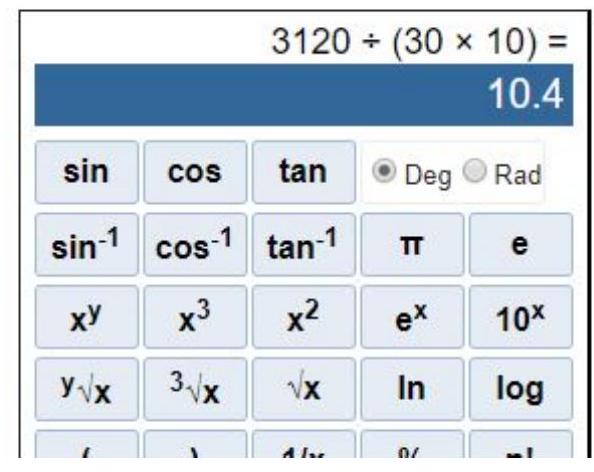
\includegraphics[max width=\textwidth]{2022_10_14_fef65bffdeb472549abeg-07}

Parenthesis () matter!!

\section{Backwash Rise Rate}
Backwash rate is occasionally measured as the upward velocity of the water during backwashing, expressed as in/min rise. To convert from $\mathrm{gpm} / \mathrm{ft}^{2}$ backwash rate to an in/min rise rate, use either of the following equations:

Backwash rate, in $/ \mathrm{min}=$ Backwash rate, $\mathrm{gpm} / \mathrm{ft}^{2} \times 1.6$

Backwash rate, in $/ \mathrm{min}=\frac{\text { Backwash rate, } \mathrm{gpm} / \mathrm{ft}^{2} \times 12 \mathrm{in} / \mathrm{ft}}{7.48 \mathrm{gal} / \mathrm{ft}^{3}}$

\section{Example:}
A filter $22 \mathrm{ft}$ long by $12 \mathrm{ft}$ wide has a backwash rate of $3260 \mathrm{gpm}$. What is this backwash rate expressed as a in/min rise?

First calculate the backwash rate as $\mathrm{gpm} / \mathrm{ft}^{2}$ :\\
Backwash rate $=\frac{\text { Flow rate, } \mathrm{gpm}}{\text { Filter area, } \mathrm{ft}^{2}}$\\
Backwash rate $=\frac{3260 \mathrm{gpm}}{22 \mathrm{ft} \times 12 \mathrm{ft}}$\\
Backwash rate $=12.3 \mathrm{gpm} / \mathrm{ft}^{2}$

Then covert $\mathrm{gpm} / \mathrm{ft}^{2}$ to the $\mathrm{in} / \mathrm{min}$ rise rate: Backwash rate, in $/ \min =\frac{\text { Backwash rate, } \mathrm{gpm} / \mathrm{ft}^{2} \times 12 \mathrm{in} / \mathrm{ft}}{7.48 \mathrm{gal} / \mathrm{ft}^{3}}$

Backwash rate, in $/ \min =\frac{12.3 \mathrm{gpm} / \mathrm{ft}^{2} \times 12 \mathrm{in} / \mathrm{ft}}{7.48 \mathrm{gal} / \mathrm{ft}^{3}}$

Backwash rate, in $/ \mathrm{min}=19.7 \mathrm{in} / \mathrm{min}$

\section{Volume of Backwash Water Required}
To determine the volume of water required for backwashing, we must know both the desired backwash flow rate, in gpm, and the duration of backwash, in minutes.

Water volume, gal $=$ Backwash flow rate, $g p m \times$ Backwash duration time, min

\section{Example:}
For a backwash flow rate of 9000 gpm and a total backwash time of 8 minutes, how many gallons of water will be required for backwashing?

Water volume, gal $=$ Backwash flow rate, gpm x Backwash duration time, min

Water volume, gal $=9000 \mathrm{gpm} \times 8 \mathrm{~min}$

Water volume, gal $=72,000$ gal

\section{Required Depth of Backwash Water Tank}
The required depth of water in the backwash water tank is determined from the volume of water required for backwashing. To make this calculation use the following equation:

Volume, gal $=0.785 \times(\text { Diameter })^{2} \times$ Depth, $\mathrm{ft} \times 7.48 \mathrm{gal} / \mathrm{ft}^{3}$

\section{Example:}
The volume of water required for backwashing has been calculated to be 85,000 gal. What is the required depth of water in the backwash water tank to provide this amount of water if the diameter of the tank is $60 \mathrm{ft}$ ?

Use the volume equation for a cylindrical tank, filling in known data, then solve for $\mathrm{x}$ :
$$
\begin{aligned}
&\text { Volume, gal }=0.785 \times(\text { Diameter })^{2} \times \text { Depth, } \mathrm{ft} \times 7.48 \text { gal } / \mathrm{ft}^{3} \\
&85,000 \mathrm{gal}=0.785 \times(60 \mathrm{ft})^{2} \times ? \text { Depth, } \mathrm{ft} \times 7.48 \mathrm{gal} / \mathrm{ft}^{3}
\end{aligned}
$$
Now you need to get the depth on one side by itself so you can solve for it. To do this you can take all of the other figures on the right hand side of the equation and move them to the left hand side. To do this you will have to divide both sides by the same. This leaves the equation looking like:

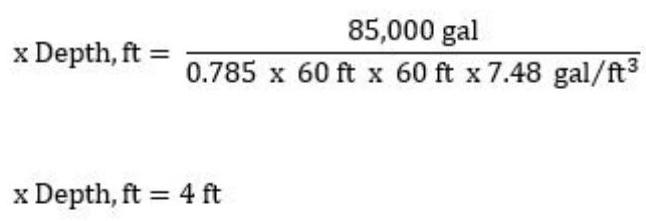
\includegraphics[max width=\textwidth]{2022_10_14_fef65bffdeb472549abeg-09}

\section{Backwash Pumping Rate}
The desired backwash pumping rate, gpm, for a filter depends on the desired backwash rate in $\mathrm{gpm} / \mathrm{ft}^{2}$ and the $\mathrm{ft}^{2}$ area of the filter. The backwash pumping rate, gpm, can be determined by using the following equation:

Pumping rate, gpm $=$ Backwash rate, $\mathrm{gpm}^{\mathrm{ftt}}{ }^{2} \mathrm{x}$ Filter area, $\mathrm{ft}^{2}$

\section{Example:}
The desired backwash pumping rate for a filter is $12 \mathrm{gpm} / \mathrm{ft}^{2}$. If the filter is $20 \mathrm{ft}$ long by $20 \mathrm{ft}$ wide, what backwash pumping rate, gpm, will be required?

Pumping rate, gpm $=$ Backwash rate, $\mathrm{gpm} / \mathrm{ft}^{2} \mathrm{x}$ Filter area, $\mathrm{ft}^{2}$

Pumping rate, gpm $=12 \mathrm{gpm} / \mathrm{ft}^{2} \times(20 \mathrm{ft} \times 20 \mathrm{ft})$

Pumping rate, gpm $=4800 \mathrm{gpm}$

\section{Percent Product Water Used for Backwashing}
Along with measuring filtration rate and filter run time, another aspect of filter operation that is monitored for filter performance is the percent of product water used for backwashing. The equation for percent of product water used for backwashing calculations used is shown as:
$$
\text { Backwash water, } \%=\frac{\text { Backwash water, gal }}{\text { Water filtered, gal }} \times 100
$$

\section{Example:}
A total of $11,400,000$ gal of water was filtered during a filter run. If backwashing used 48,500 gal of this product water, what percent of the product water is used for backwashing?

Backwash water, $\%=\frac{\text { Backwash water, gal }}{\text { Water filtered, gal }} \times 100$

Backwash water, $\%=\frac{48,500 \text { gal }}{11,400,000 \text { gal }} \times 100$

Backwash water, $\%=0.43 \%$

\section{Percent Mud Ball Volume}
Mud balls are heavier deposits of solids near the top surface of the medium that break into pieces during backwash, resulting in spherical accretions of floc and sand (usually less than 12 inches in diameter). The presence of mud balls in the filter media is checked periodically. The principal objection to mud balls is that they diminish the effective filter area. The percent mud ball volume can be determined by:

Mud ball volume, $\%=\frac{\text { Mud ball volume, } \mathrm{mL}}{\text { Total sample volume, } \mathrm{mL}} \times 100$

\section{Example:}
A filter is tested for the presence of mud balls. The mud ball sample has a total sample volume of $680 \mathrm{~mL}$. Five samples were taken from the filter. When the mud balls were placed in $500 \mathrm{~mL}$ of water, the water level rose to $565 \mathrm{~mL}$. What is the percent mud ball volume of the sample?

The mud ball volume needed for the equation is the volume that the water rose:

$565 \mathrm{~mL}-500 \mathrm{~mL}=65 \mathrm{~mL}$

Because 5 samples of media were taken, the total sample volume is 5 times the sample volume:

$5 \times 680 \mathrm{~mL}=3400 \mathrm{~mL}$

Now plug the values into the formula:

Mud ball volume, $\%=\frac{\text { Mud ball volume, } \mathrm{mL}}{\text { Total sample volume, } \mathrm{mL}} \times 100$

Mud ball volume, $\%=\frac{65 \mathrm{~mL}}{3400 \mathrm{~mL}} \times 100$

Mud ball volume, $\%=1.9 \%$

\section{Filter Bed Expansion}
In addition to backwash rate, it is also important to expand the filter media during the wash to maximize the removal of particles held in the filter or by the media; that is, the efficiency of the filter wash operation depends on the expansion of the sand bed. Bed expansion is determined by measuring the distance from the top of the unexpanded media to a reference point (i.e. top of the filter wall) and from the top of the expanded media to the same reference. A proper backwash rate should expand the filter 20 to $25 \%$. Percent bed expansion is given by dividing the bed expansion by the total depth of expandable media (i.e. media depth less support gravels) and multiplied by 100 , as follows:

Expanded measurement $=$ Depth to top of media during backwash, inches

Unexpanded measurement $=$ Depth to top of media before backwash, inches

Bed expansion $=$ Unexpanded measurement, inches - Expanded measurement, inches Bed expansion, $\%=\frac{\text { Bed expansion, in }}{\text { Total expandable media depth, in }} \times 100$

\section{Example:}
The backwashing practices for a filter with 30 inches of anthracite and sand are being evaluated. While at rest, the distance from the top of the media to the concrete floor surrounding the top of filter is measured to be 41 inches. After the backwash has begun and the maximum backwash rate is achieved, a probe containing a white disk is slowly lowered into the filter bed until anthracite is observed on the disk. The distance from the expanded media to the concrete floor is measured to be $34.5$ inches. What is the percent bed expansion?

Given:

Unexpanded measurement $=41$ inches

Expanded measurement - $34.5$ inches

Bed expansion $=$ Unexpanded measurement, inches $-$ Expanded measurement, inches

Bed expansion $=41$ inches $-34.5$ inches

Bed expansion $=6.5$ inches

Bed expansion, $\%=\frac{\text { Bed expansion, in }}{\text { Total expandable media depth, in }} \times 100$

Bed expansion, $\%=\frac{6.5 \text { in }}{30 \text { in }} \times 100$

Bed expansion, $\%=22 \%$

\section{Review}
Water filtration is a physical process of separating suspended and colloidal particles from water by passing water through a granular material. The process of filtration involves straining, settling, and adsorption. As floc passes into the filter, the spaces between the filter grains become clogged, reducing this opening and increasing removal. Some material is removed merely because it settles on a media grain. One of the most important processes is adsorption of the floc onto the surface of individual filter grains. This helps collect the floc and reduces the size of the openings between the filter media grains. In addition to removing silt and sediment, floc, algae, insect larvae, and any other large elements, filtration also contributes to the removal of bacteria and protozoa such as Giardia lamblia and Cryptosporidium. Some filtration processes are also used for iron and manganese removal. Filtration is the mechanical removal of turbidity particles by passing the water through a porous medium, which is either a granular bed or a membrane. Filtration's purpose is to remove all the turbidity particles carried over from the sedimentation phase, thus producing a sparkling clear water with almost zero turbidity.

\section{Assignment}
Please complete the math worksheet for this lesson. You will need to be logged into Canvas to complete this assignment. Make sure you choose the appropriate semester.


\end{document}